\documentclass{beamer}
\usetheme{CambridgeUS}
\usepackage[utf8]{inputenc}
\usepackage{tikz}
\usetikzlibrary{quotes} % LATEX and plain TEX
\usetikzlibrary{arrows,automata,positioning}

\usetikzlibrary{shapes.geometric}
\usetikzlibrary{snakes}



\title{1-2-3 Domneva}

\author{Gašper Domen Romih}

\date{\today}

\begin{document}
\begin{frame}
	\titlepage
\end{frame}
\begin{frame}
\tableofcontents
\end{frame}
\section{Osnovne definicije}

\begin{frame}
\begin{block}{Graf}
Graf $G$ je urejen par $(V, E)$, kjer je množica $V$ množice vozlišč in $E \subset V^2$ množice povezav.
\end{block}

\begin{block}{Barvanje grafa}
	Barvanje grafa $G = (V, E)$ je preslikava $c : V \rightarrow S$. Množici $S$ rečemo množica barv. Rečemo, da je barvanje \textbf{pravilno}, če za vsak $uv \in E$ velja $c(u) \neq c(v)$.
\end{block}
\begin{block}{Utežitev grafa}
	Utežitev grafa je preslikava $\omega : E \rightarrow W$. V kolikor je množica uteži $W$ oblike $\{1,2,\ldots, k\}$ rečemo, da je preslikava $\omega$ $k$-utežitev grafa $G$.
\end{block}
\end{frame}

\begin{frame}{Od utežitve do barvanja}
\begin{block}{Barvanje grafa z $k$-utežitvijo}
	Naj bo $\omega$ neka $k$-utežitev grafa $G$. Sedaj definiramo preslikavo $c_{\omega} : V \rightarrow S$ na naslednji način:
	$$ c_{\omega}(u) = \sum_{e = uv \in E} \omega(e). $$
\end{block}
\begin{figure}
			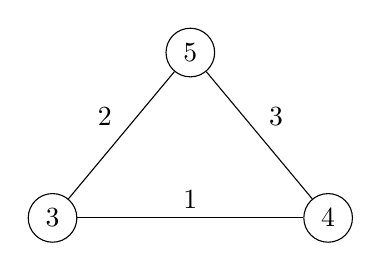
\begin{tikzpicture}
	[scale=.7,auto=left,main node/.style={shape=circle,draw,fill=white}]
	\node [main node] (1) at (0,0) {3};
	\node [main node] (2) at (5,0) {4};
	\node [main node] (3) at (2.5,3) {5};
	
	
	\path[]
	(1) edge node {1} (2)
	(1) edge node {2} (3)
	(2) edge node [above right] {3} (3)
	
	;
	
	
	
	\end{tikzpicture}
	\caption{Primer $3$-utežitve, ki porodi pravilno $3$-barvanje.}
\end{figure}

\end{frame}

\section{1-2-3 Domneva}
\begin{frame}
\begin{block}{}
	Označimo z $\mu(G)$ najmanjši tak $k$ za katerega obstaja $k$-utežitev $\omega$ grafa $G$, ki inducira pravilno barvanje $c_{\omega}$.
\end{block}
\begin{block}{1-2-3 Domneva}
	Za vsak povezan graf $G$, ki ni $K_2$ je $\mu(G) \le 3$.
\end{block}
\end{frame}

\subsection{Zgodovinski okvir}
\begin{frame}
\begin{itemize}
	\item Leta 2004 v članku [] zastavljena domneva.
	\item Leta 2007 dokazano $\mu(G) \le 30$.
	\item Leta 2008 dokazano $\mu(G) \le 16$.
	\item Leta 2008 dokazano $\mu(G) \le 13$.
	\item Leta 2009 $\mu(G) \le 6$.
	\item Leta 2010 $\mu(G) \le 5$. To je do sedaj tudi najboljši rezultat za splošne grafe.
\end{itemize}

\begin{block}{Opomba}
	Kljub temu, da je trenutno najboljša zgornja $\mu(G) \le 5$ je za veliko zananih družin grafov dokazano $\mu(G) \le 3$. 
\end{block}
\end{frame}

\begin{frame}{Pristopi k 1-2-3 domnevi}
V teoriji grafov domneve in podobne probleme obravnavamo na več različnih načinov. Nekaj metod in pristopov:
\begin{itemize}
	\item Direktno poizkušamo dokazati oziroma zavreči domnevo.
	\item Pokažemo, da domneva velja za znane družine grafov ($P_n, C_n, K_n, \ldots$).
	\item Pokažemo, da domneva velja za grafe z nekimi dodatnimi lastnostmi (dvodelni, 3-obarljivi, $\ldots$).
	\item Pokažemo, da velja neka bolj \textit{omiljena} verzija domneve. Npr. $\mu(G) \le 5$.
	
	\item Verjetnostne metode lahko dokažejo domnevo za dovolj \textit{velike} grafe.
	
\end{itemize}
\end{frame}

\subsection{Izračun $\mu$ za poti}
\begin{frame}{$\mu(P_n)$ za $n \le 3$}
V primeru $n=2$ imamo graf $K_n$ zato obravnavamo primere ko $n \ge 3$.  Posebaj si oglejmo še primer ko $n = 3$.  V tem primeru utežimo povezavi z $1$ in dobimo pravilno barvanje iz česar sledi $\mu(P_3) = 1$.

\begin{figure}[!h]
	\centering
	\label{fig:pn}
	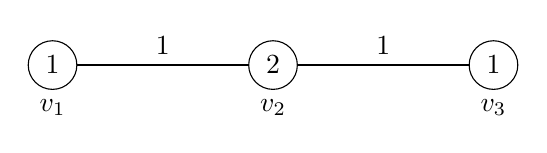
\begin{tikzpicture}
	[scale=.7,auto=left,main node/.style={shape=circle,draw,fill=white}]
	\node [main node] (1) at (1,1) [label=below:$v_1$] {1} ;
	\node [main node](2) at (5,1) [label=below:$v_2$] {2} ;
	\node [main node](3) at (9,1) [label=below:$v_3$] {1} ;
	
	
	\path[draw,thick]
	(1) edge node {1} (2)
	(2) edge  node {1} (3)
	
	;
	
	\end{tikzpicture}
	\caption{Primer utežitve grafa $P_n$.}
\end{figure}
\end{frame}

\begin{frame}{$\mu(P_n)$ za $n > 3$}
	Najprej oštevilčimo povezave kot $e_1, e_2, \ldots, e_{n-1}$, kjer $e_i = v_i v_{i+1}$ za $1 \le i < n$.
	\begin{block}{Pogoj za pravilno barvanje}
		Utežitev povezav $\omega$ inducira pravilno barvanje $P_n$ natanko tedaj ko $\omega(e_i) \neq \omega(e_j)$ za vsak $|j -i| = 2$.
	\end{block}
\begin{figure}[!h]
	\centering
	\label{fig:pn}
	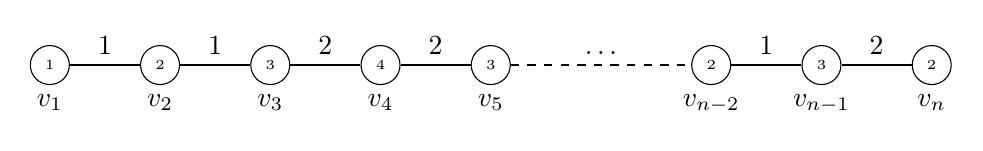
\begin{tikzpicture}
	[scale=.7,auto=left,main node/.style={shape=circle,draw,fill=white}]
	\node [main node] (1) at (1,1) [label=below:$v_1$] {\tiny 1} ;
	\node [main node](2) at (3,1) [label=below:$v_2$] {\tiny 2} ;
	\node [main node](3) at (5,1) [label=below:$v_3$] {\tiny 3} ;
	\node [main node](4) at (7,1) [label=below:$v_4$] {\tiny 4} ;
	\node [main node](5) at (9,1) [label=below:$v_5$] {\tiny 3} ;
	
	\node [main node](6) at (13,1) [label=below:$v_{n-2}$] {\tiny 2} ;
	\node [main node](7) at (15,1) [label=below:$v_{n-1}$] {\tiny 3} ;
	\node [main node](8) at (17,1) [label=below:$v_n$]  {\tiny 2};
	
	
	\path[draw,thick]
	(1) edge node {1} (2)
	(2) edge  node {1} (3)
	(3) edge  node {2} (4)
	(4) edge  node {2} (5)
	
	(5) edge [dashed]  node {$\ldots$} (6)
	
	(6) edge  node {1} (7)
	(7) edge  node {2} (8)
	;
	
	\end{tikzpicture}

\end{figure}
\end{frame}

\begin{frame}{Ugotovitve za $P_n$}
	\begin{block}{Utežitev $\omega$ za $P_n$}
		$$
		\omega(e_i) = \begin{cases}
			1 &i \equiv 1,2 \pmod{4}\\ 
			2 &i \equiv 3,4 \pmod{4}
		\end{cases}
		$$
	\end{block}
	\begin{itemize}
		\item Našli smo $2$-utežitev, ki porodi pravilno barvanje $\implies$  $\mu(P_n) = 2$.
		\item Zaporedje uteži na povezavah je $11221\ldots 22112$, lahko pa bi definicijo utežitve popravili z naprimer levim zamikom zgornjega zaporedja. To so tudi vse možne pravilne $2$-utežitve poti.
	\end{itemize}
\end{frame}

\subsection{Izračun $\mu$ za cikle}
\begin{frame}{Osnovna ideja za izračun $\mu(C_n)$}
	\begin{block}{Ideja}
		Cikel je pot, ki ji dodamo povezavo $e_n$ med prvim in zadnjih vozliščem. Pogoj za pravilno barvanje poti velja tudi za cikle . Poizkusili bomo modificirati obstoječo utežitev za poti, tako da boveljavna tudi za cikle.
	\end{block}

\begin{figure}
	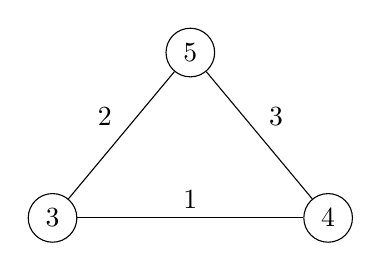
\begin{tikzpicture}
	[scale=.7,auto=left,main node/.style={shape=circle,draw,fill=white}]
	\node [main node] (1) at (0,0) {3};
	\node [main node] (2) at (5,0) {4};
	\node [main node] (3) at (2.5,3) {5};
	
	
	\path[]
	(1) edge node {1} (2)
	(1) edge node {2} (3)
	(2) edge node [above right] {3} (3)
	
	;
	
	
	
	\end{tikzpicture}
	\caption{Na primeru $C_3$ vidimo, $\mu(C_3) = 3$, saj morajo v luči potrebnega pogaja uteži na povezavah biti paroma različne.}
\end{figure}
\end{frame}

\begin{frame}{$\mu(C_n)$ za $n = 4k$}
	Vzamemo kar enako utežitev kot za pot, z dodatkom $\omega(e_n) = 2$.
	\begin{figure}
		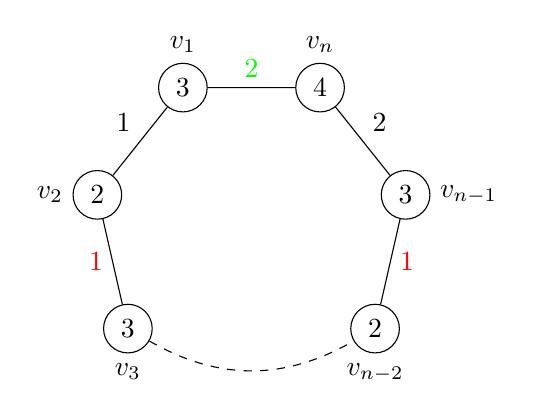
\begin{tikzpicture}
		
		[scale=.8,auto=left,main node/.style={draw=none,fill=none}]
		\def \n {7}
		\node[
		regular polygon,
		regular polygon sides=\n,
		minimum size=4cm,
		rotate=180/\n,
		] (a) {};
		
		\node[draw,shape=circle,fill=none] (1) at (a.corner 1) [label=above:$v_1$] { $3$};
		\node[draw,shape=circle,fill=none] (2) at (a.corner 2) [label=left:$v_2$] { $2$};
		\node[draw,shape=circle,fill=none] (3) at (a.corner 3) [label=below:$v_3$]{ $3$};
		
		\node[draw,shape=circle,fill=none] (4) at (a.corner 5) [label=below:$v_{n-2}$] { $2$};
		\node[draw,shape=circle,fill=none] (5) at (a.corner 6) [label=right:$v_{n-1}$] { $3$};
		\node[draw,shape=circle,fill=none] (6) at (a.corner 7) [label=above:$v_n$]{ $4$};
		
		\draw[] (1) to node [above left] {1}  (2);
		\draw[] (2) to node [text=red,left] {1}  (3);
		\draw[bend right, dashed] (3) to node [] {}  (4);
		\draw[] (4) to node [text=red, right] {1}  (5);
		\draw[] (5) to node [above right] {2}  (6);
		
		\draw[] (6) to node [text=green,above] {2}  (1);
		\end{tikzpicture}
		\caption{Kot je razvidno iz slike zgornja utežitev porodi pravilno barvanje. Na povezavo $e_n$ (označena rdeče) tako vplivata le povezavi $e_2$ in $e_{n-2}$ (označena zeleno). Iz tega sledi $\mu(c_{4k}) = 2$.}
	\end{figure}
\end{frame}

\begin{frame}{$\mu(C_n)$ za $n = 4k + 1$}
Ponovno vzamemo utežitev za pot ter dodamo $\mu(e_n) = 3$.
	\begin{figure}
	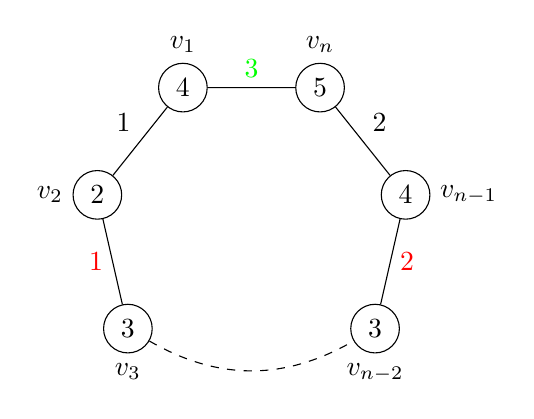
\begin{tikzpicture}
	
	[scale=.8,auto=left,main node/.style={draw=none,fill=none}]
	\def \n {7}
	\node[
	regular polygon,
	regular polygon sides=\n,
	minimum size=4cm,
	rotate=180/\n,
	] (a) {};
	
	\node[draw,shape=circle,fill=none] (1) at (a.corner 1) [label=above:$v_1$] { $4$};
	\node[draw,shape=circle,fill=none] (2) at (a.corner 2) [label=left:$v_2$] { $2$};
	\node[draw,shape=circle,fill=none] (3) at (a.corner 3) [label=below:$v_3$]{ $3$};
	
	\node[draw,shape=circle,fill=none] (4) at (a.corner 5) [label=below:$v_{n-2}$] { $3$};
	\node[draw,shape=circle,fill=none] (5) at (a.corner 6) [label=right:$v_{n-1}$] { $4$};
	\node[draw,shape=circle,fill=none] (6) at (a.corner 7) [label=above:$v_n$]{ $5$};
	
	\draw[] (1) to node [above left] {1}  (2);
	\draw[] (2) to node [text=red,left] {1}  (3);
	\draw[bend right, dashed] (3) to node [] {}  (4);
	\draw[] (4) to node [text=red, right] {2}  (5);
	\draw[] (5) to node [above right] {2}  (6);
	
	\draw[] (6) to node [text=green,above] {3}  (1);
	\end{tikzpicture}
	\caption{Kot je razvidno iz slike zgornja utežitev porodi pravilno barvanje. Nova povezava sedaj zaradi omejitev ne more imeti uteži $1$ ali $2$. Utež 3 na povezavi $e_n$ tako porodi pravilno barvanje iz česar sledi $\mu(C_{4k + 1}) \le 3$.}
\end{figure}
\end{frame}

\begin{frame}{$\mu(C_n)$ za $n=4k + 2$}
	Poleg povezave $e_n$ moramo v tem primeru popravit tudi $e_{n-1}$.
	
		\begin{figure}
		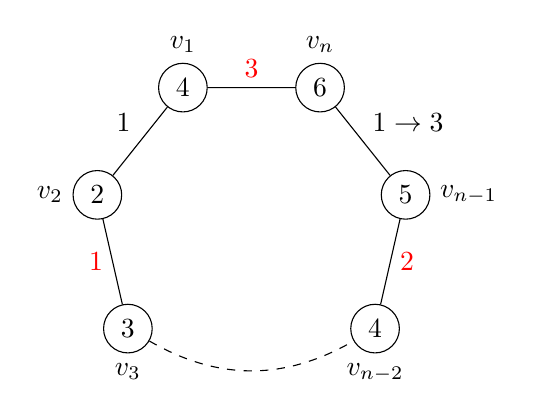
\begin{tikzpicture}
		
		[scale=.8,auto=left,main node/.style={draw=none,fill=none}]
		\def \n {7}
		\node[
		regular polygon,
		regular polygon sides=\n,
		minimum size=4cm,
		rotate=180/\n,
		] (a) {};
		
		\node[draw,shape=circle,fill=none] (1) at (a.corner 1) [label=above:$v_1$] { $4$};
		\node[draw,shape=circle,fill=none] (2) at (a.corner 2) [label=left:$v_2$] { $2$};
		\node[draw,shape=circle,fill=none] (3) at (a.corner 3) [label=below:$v_3$]{ $3$};
		
		\node[draw,shape=circle,fill=none] (4) at (a.corner 5) [label=below:$v_{n-2}$] { $4$};
		\node[draw,shape=circle,fill=none] (5) at (a.corner 6) [label=right:$v_{n-1}$] { $5$};
		\node[draw,shape=circle,fill=none] (6) at (a.corner 7) [label=above:$v_n$]{ $6$};
		
		\draw[] (1) to node [above left] {1}  (2);
		\draw[] (2) to node [text=red,left] {1}  (3);
		\draw[bend right, dashed] (3) to node [] {}  (4);
		\draw[] (4) to node [text=red, right] {2}  (5);
		\draw[] (5) to node [above right] {$1 \to 3$}  (6);
		
		\draw[] (6) to node [text=red,above] {3}  (1);
		\end{tikzpicture}
		\caption{Kot v prjšnjem primer moramo nastavit utež na povezavi $e_n$ na 3. Ker ima povezava $e_1$ enako utež kot $e_{n-1}$ popravimo še utež na tej povezavi na 3. }
	\end{figure}
\end{frame}

\begin{frame}{$\mu(C_n)$ za $n = 4k + 3$}
	V tem primeru moramo prav tako popravit uteži na dveh povezavah. Deluje kar isti popravek kot v prejšnjem primeru.
	
		\begin{figure}
		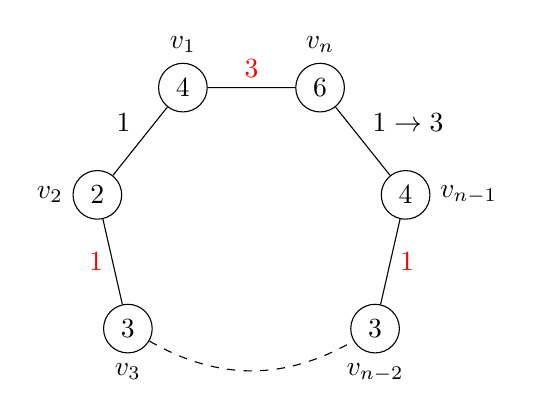
\begin{tikzpicture}
		
		[scale=.8,auto=left,main node/.style={draw=none,fill=none}]
		\def \n {7}
		\node[
		regular polygon,
		regular polygon sides=\n,
		minimum size=4cm,
		rotate=180/\n,
		] (a) {};
		
		\node[draw,shape=circle,fill=none] (1) at (a.corner 1) [label=above:$v_1$] { $4$};
		\node[draw,shape=circle,fill=none] (2) at (a.corner 2) [label=left:$v_2$] { $2$};
		\node[draw,shape=circle,fill=none] (3) at (a.corner 3) [label=below:$v_3$]{ $3$};
		
		\node[draw,shape=circle,fill=none] (4) at (a.corner 5) [label=below:$v_{n-2}$] { $3$};
		\node[draw,shape=circle,fill=none] (5) at (a.corner 6) [label=right:$v_{n-1}$] { $4$};
		\node[draw,shape=circle,fill=none] (6) at (a.corner 7) [label=above:$v_n$]{ $6$};
		
		\draw[] (1) to node [above left] {1}  (2);
		\draw[] (2) to node [text=red,left] {1}  (3);
		\draw[bend right, dashed] (3) to node [] {}  (4);
		\draw[] (4) to node [text=red, right] {1}  (5);
		\draw[] (5) to node [above right] {$1 \to 3$}  (6);
		
		\draw[] (6) to node [text=red,above] {3}  (1);
		\end{tikzpicture}
		\caption{Na enak način kot v prejšnjem primeru dobimo pravilno barvanje. }
	\end{figure}
\end{frame}

\begin{frame}{Ugotovitve za $C_n$}
	Ugotovili smo, da $\mu(C_n) \le 3$ za vsak $n$. Pokazali bomo še, da je ta meja tudi stroga za $n \neq 4k$. Recimo nasprotno torej, da imamo $2$-utežitev cikla, ki porodi pravilno barvanje. Veljati mora torej $\omega(e_i) \neq \omega(e_{i + 2})$ iz česar sledi $\omega(e_i) = \omega(e_{i + 4})$. To pa je protislovje ko $n \neq 4k$.
	\begin{block}{Rezultat}
		
		Za $C_n$ velja:
		$$ 
		\mu(C_n) = 
		\begin{cases}
		2; \text{ } n \equiv 0 \pmod{4} \\
		3; \text{ sicer}
		\end{cases}
		$$
	\end{block}
\end{frame}

\section{Izrek za $k$-obarljive grafe}
\begin{frame}{Obravnavanje $k$-obarljivih grafov}
	\begin{block}{Ideja}
		Za $k$-obarljive grafe, lahko uteži gledamo modulo $k$ in še vedno dobimo veljavne rezultate. V ta namen bomo za množico uteži vzeli neko Abelovo grupo $\Gamma$, ter inducirano barvanje gledali v tej množici.
	\end{block}

	\begin{block}{Trditev}
		Naj bo $\Gamma$ Abelova grupa z $|\Gamma| = n$ in naj $0$ označuje enoto. Tedaj za vsak $g \in \Gamma$ velja $ng = 0$.
	\end{block}
\end{frame}

\begin{frame}
	\begin{block}{Trditev}
		Naj bo $\Gamma$ Abelova grupa lihe moči in $|\Gamma| = n$. Tedaj za vsak element $g \in \Gamma$ obstaja $h \in \Gamma$, tako da $g = 2h$.
	\end{block}

	\begin{block}{Dokaz}
			Ker je $\Gamma$ Abelova grupa po prejšnji trditvi vemo, da $ 0 = ng$. Prištejemo $g$ na obeh straneh in dobimo $g = (n+1)g$. Sedaj označimo $h = \frac{n + 1}{2}g$ in očitno velja $g = 2h$.
	\end{block}
\end{frame}

\begin{frame}{Izrek za $k$-obarljive grafe}
	\begin{block}{Izrek}
	Naj bo $\Gamma$ Abelova grupa lihe moči in G ne-trivialen $|\Gamma|$-barljiv graf. Potem obstaja utežitev $\omega$ z elementi iz $\Gamma$, tako da je inducirano barvanje $c_{\omega}$ pravilno.
	\end{block}

	Nekaj opomb:
	\begin{itemize}
		\item Zgornji izrek dokaže domnevo v primeru dvodelnih in splošneje $3$-obarljivih grafov. Vsak tak graf, torej lahko utežimo z naprimer $\mathcal{Z}_3 = \{0,1,2\}$.
		\item Definicija induciranega barvanje $c_{\omega}$ preko uteženih povezav je potekala na enostaven način. Kaj pa v drugo smer? Recimo, da imamo neko barvanje grafa z $k$ barvami. Zgornji izrek, oziroma njegov dokaz konstruirata utežitev z $k$ utežmi, ki inducira to barvanje (za lihe $k$).
	\end{itemize}
\end{frame}

\begin{frame}{Dokaz izreka}
	Izrek bomo dokazali, tako da bomo konstruirali ustrezno utežitev z elementi iz $\Gamma = \{g_1, g_2, \ldots, g_k\}$. Naj bo $c$ neko barvanje grafa $G$ z največ $k$ barvami in označimo z $n_i \ge 0$ število vozlišč barve $i$.
	
	Konstrukcija bo potekala v nekaj korakih:
	\begin{enumerate}
		\item Določitev začetnih uteži.
		\item Iterativno popravljamo uteži nepravilno pobarvanih vozlišč.
		\item Nakoncu moramo mord popravit utež nekega \textit{posebnega} vozlišča.
	\end{enumerate}
\end{frame}

\begin{frame}{Primer, ko $G$ ni dvodelen}
Po trditvi obstaja $h \in \Gamma$, tako da $n_1g_1 + n_2g_2 + \ldots + n_k g_k = 2h$. Sedaj na poljubno povzavo v grafu dodamo utež $h$ na vse ostale pa $0$ (enoto). Tako je vsota vseh uteži na vozliščih enaka $2h$.
\begin{figure}
	\begin{tikzpicture}
	[scale=.7,auto=left,main node/.style={shape=circle,draw,fill=white}]
	\node [main node] (1) at (0,0) {$h$};
	\node [main node] (2) at (5,1) {$h$};
	
	\node [] (3) at (7, 2) {};
	\node [] (4) at (7,0) {};
	
		\node [] (5) at (-2, 1) {};
	\node [] (6) at (-2,-1) {};	

	\path[]
	(1) edge node {$h$} (2)
	(2) edge[dashed]  node {$0$} (3)
	(2) edge[dashed]  node {$0$} (4)
		(1) edge[dashed]  node {$0$} (5)
	(1) edge[dashed]  node {$0$} (6)
	
	;
	
	
	
	\end{tikzpicture}
\end{figure}
\end{frame}

\begin{frame}{Primer, ko G ni dvodelen}
	Sedaj bomo uteži popravljali, tako da ohranjamo skupno vsoto uteži $2h$ dokler nima vsako vozlišče barve $i$ uteži $g_i$. Recimo torej, da ima vozlišče $u$ barve $i$ utež $g \neq g_i$. Zaradi simetričnosti obstaja vozlišče $v \neq u$, ki ima tudi napačno utež $x$. Sedaj najdemo sprehod sode dolžine med $u$ in $v$ kar vedno lahko nardimo v grafu, ki ni dvodelen. Povezavam na tem sprehodu izmenično prištevamo uteži: $ +(g_i - g), - (g_i - g), \ldots, -(g_i - g)$.
	\begin{figure}
		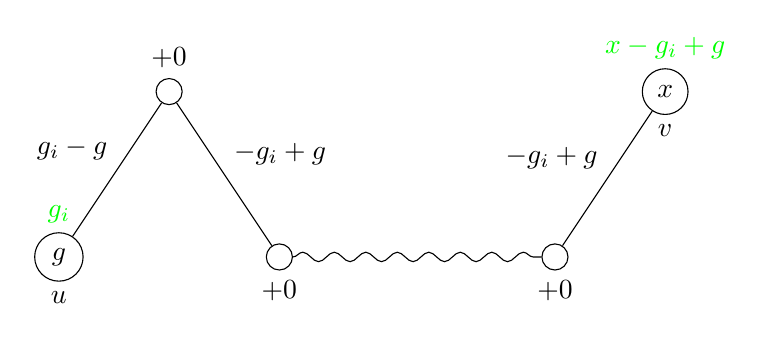
\begin{tikzpicture}
		[scale=.7,auto=left,main node/.style={shape=circle,draw,fill=white}]
		\node [main node][label=below:$u$][label=above:\textcolor{green}{$g_i$}] (1) at (0,0) {$g$};
		\node [main node][label=above:$+0$] (2) at (2,3) {};		
		\node [main node][label=below:$+0$] (3) at (4, 0) {};
		
	
		
		\node [main node][label=below:$+0$] (6) at (9, 0) {};
		\node [main node][label=below:$v$][label=above:\textcolor{green}{$x - g_i + g$}] (7) at (11,3) {$x$};	
		
		\tikzset{decoration={snake,amplitude=.6mm,segment length=4mm,
				post length=0mm,pre length=0mm}}
		
		
		\path[]
		(1) edge node {$g_i - g$} (2)
		
		(2) edge  node {$-g_i + g$} (3)
		(3) edge[decorate]  node {} (6)
		
		(6) edge  node {$-g_i + g$} (7)
		
		;
		
		
		
		\end{tikzpicture}
	\end{figure}
\end{frame}

\begin{frame}{Primer, ko G ni dvodelen}
	Nekaj opomb na zgornji postopek:
	\begin{itemize}
		\item Na vsakem koraku se ohranja skupna vsota uteži $2h$.
		\item Na vsakem koraku, imamo vsaj eno vozlišče več, ki ima pravilno utež.
	\end{itemize}

	Sklepamo torej, da nas tak postopek pripelje do pravilne utežitve grafa $G$. Oglejmo si sedaj še primer, ko je $G$ dvodelen.
\end{frame}

\begin{frame}{$G$ dvodelen}
Ker je graf dvodelen ima dva barvna razreda, vendar v tem primeru ne moremo vedno zagotoviti, da bodo uteži na vozliščih konstantne znotraj teh dveh razredov. Zato izberimo barvo $1$, tako da obstaja vozlišče  $x$ barve $1$ in je stopnje vsaj $2$. Izberemo še $2h = g_1 \neq 0 = g_2$.

	\begin{figure}
	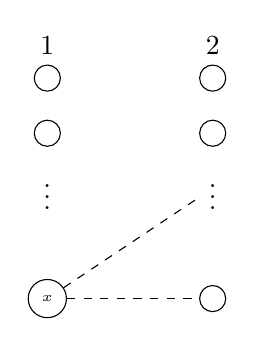
\begin{tikzpicture}
	[scale=.7,auto=left,main node/.style={shape=circle,draw,fill=white}
	]
	

	\node [main node][label=above:$1$] (1) at (0, 5) {};
	\node [main node] (2) at (0,4) {};
	\node [draw=none] (7) at (0, 3) {$\vdots$};
	\node [main node] (3) at (0,1) {\tiny $x$};  
	
	\node [main node][label=above:$2$] (4) at (3, 5) {};
	\node [main node] (5) at (3,4) {};
	\node [draw=none] (8) at (3, 3) {$\vdots$};
	\node [draw=none] (9) at (3, 2) {};
	\node [main node] (6) at (3,1) {};
	  
	\path[]
	(3) edge[dashed] node {} (8)
	(3) edge[dashed] node {} (6)	
	;
	
	\end{tikzpicture}
\end{figure}
\end{frame}

\begin{frame}{G dvodelen}
	Sedaj nadaljujemo podobno kot prej in na vse povezave damo utež 0 ($=g_2$). Uteži popravljamo podobno kot prej. Za vsak $u \neq x$ iz barvnega razreda $1$, ki ima utež $0$ najdemo pot sode dolžine od $u$ do $x$ in popravljamo uteži z $g1, -g1, \ldots, -g_1$.
	
		\begin{figure}
		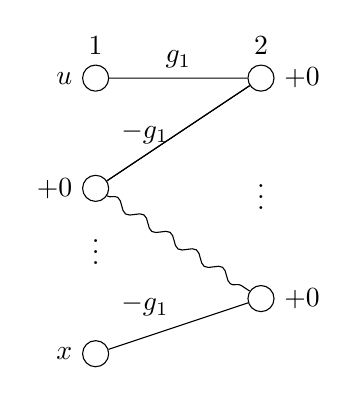
\begin{tikzpicture}
		[scale=.7,auto=left,main node/.style={shape=circle,draw,fill=white}
		]
		
		
		\node [main node][label=above:$1$][label=left:$u$] (1) at (0, 6) {};
		\node [main node][label=left:$+0$] (2) at (0,4) {};
		\node [draw=none] (7) at (0, 3) {$\vdots$};
		\node [main node][label=left:$x$] (3) at (0,1) {};  
		
		\node [main node][label=above:$2$][label=right:$+0$] (4) at (3, 6) {};
		
		\node [draw=none] (8) at (3, 4) {$\vdots$};
		\node [main node][label=right:$+0$] (9) at (3, 2) {};
	  	
			
		\tikzset{decoration={snake,amplitude=.6mm,segment length=4mm,
				post length=0mm,pre length=0mm}}
		\path[]
		(1) edge node {$g_1$} (4)
		(4) edge node[ left] {$-g_1$} (2)
		(4) edge node {} (2)
		(2) edge[decorate] node {} (9)
		
		(3) edge[] node {$-g_1$} (9)	
		;
		
		\end{tikzpicture}
	\end{figure}
\end{frame}
\begin{frame}{G dvodelen}
	Po končanem postopku imajo vsa vozlišča v razredu $2$ utež $0$. Vozlišča v razredu $1$ imajo utež $g_1$ razen vozlišča $x$, ki ima utež $-(n_1 - 1)g_1$. V kolikor $-(n_1 - 1)g_1 \neq 0$ smo končali. V nasprotnem primeru na poljubni 2 povezavi, ki gresta iz $x$ dodamo utež $h$.
	
			\begin{figure}
		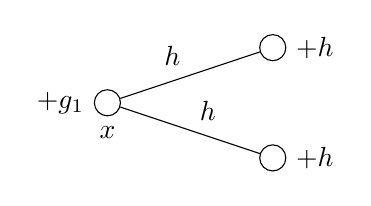
\begin{tikzpicture}
		[scale=.7,auto=left,main node/.style={shape=circle,draw,fill=white}
		]
		
		
		\node [main node][label=below:$x$][label=left:$+g_1$] (1) at (0, 1) {};
		\node [main node][label=right:$+h$] (2) at (3,2) {};
		\node [main node][label=right:$+h$] (3) at (3,0) {};

		
		
		
		\path[]
		(1) edge node {$h$} (2)
		
		(1) edge node {$h$} (3)	
		
		;
		
		\end{tikzpicture}
	\end{figure}

Tako imamo v razredu $1$ vsa vozlišča z utežjo $g_1$ medtem ko imamo v razredu $2$ vozlišča z utežmi $g_2 = 0$ in $h \neq g_1$. S tem je izrek dokazan.
	
\end{frame}



\end{document}